\chapter{Results}
\label{ch:Results}
We show the results of the different experiments and discuss their implications.

\section{Hyperparameter Search}
We list the selected learning rate and regularization parameter for the five folds of each experiment (Tab~\ref{tab:HSResults}). Although hyperparameters were selected independently in each fold, they converge to similar values for the same experiment.
\begin{table}[h]
	\centering
	\setlength\tabcolsep{3.5pt}
	\begin{tabular}{l*{10}{c}}
		\hline
		 & \multicolumn{2}{c}{\textbf{Fold 1}} & \multicolumn{2}{c}{\textbf{Fold 2}} &\multicolumn{2}{c}{\textbf{Fold 3}} &\multicolumn{2}{c}{\textbf{Fold 4}} &\multicolumn{2}{c}{\textbf{Fold 5}}\\
		& \textbf{$\alpha$} & \textbf{$\lambda$} & \textbf{$\alpha$} & \textbf{$\lambda$} & \textbf{$\alpha$} & \textbf{$\lambda$} & \textbf{$\alpha$} & \textbf{$\lambda$} & \textbf{$\alpha$} & \textbf{$\lambda$}\\
		\hline 
		Exp. 1.1	&\sn{2}{-4}	&\sn{3}{-2}	&\sn{2}{-4}	&\sn{4}{-2}	&\sn{9}{-5}	&\sn{5}{-3}	&\sn{6}{-4}	&\sn{8}{-3}	&\sn{6}{-4}	&\sn{1}{-2}\\
		Exp. 1.2	&\sn{4}{-4}	&\sn{9}{-2}	&\sn{4}{-4}	&\sn{5}{-2}	&\sn{4}{-4}	&\sn{7}{-3}	&\sn{3}{-4}	&\sn{5}{-3}	&\sn{6}{-4}	&\sn{3}{-2}\\
		Exp. 1.3	&\sn{4}{-4}	&\sn{3}{-2}	&\sn{2}{-4}	&\sn{4}{-2}	&\sn{7}{-5}	&\sn{6}{-3}	&\sn{4}{-4}	&\sn{8}{-2}	&\sn{8}{-4}	&\sn{3}{-2}\\
		Exp. 2		&\sn{1}{-5}	&\sn{4}{-4}	&\sn{5}{-5}	&\sn{4}{-3}	&\sn{5}{-5}	&\sn{1}{-3}	&\sn{1}{-5}	&\sn{2}{-4}	&\sn{5}{-5}	&\sn{2}{-4}\\
		Exp. 3		&\sn{1}{-4}	&\sn{4}{-4}	&\sn{7}{-5}	&\sn{5}{-4}	&\sn{1}{-4}	&\sn{7}{-4}	&\sn{7}{-5}	&\sn{2}{-4}	&\sn{8}{-5}	&\sn{9}{-5}\\
		\hline
	\end{tabular}
	\caption[Selected hyperparameters]{Selected learning rate and regularization parameter configurations.}
	\label{tab:HSResults}
\end{table}

\section{Experiments}
Models perform similarly while commiting few errors (Fig.~\ref{fig:FROCResults}): different models perform better at different false positive per image marks but overall diferences are small. Furthermore, performance varies significantly among different folds of the same experiment making inferences harder.
\begin{figure}[h]
	\centering
		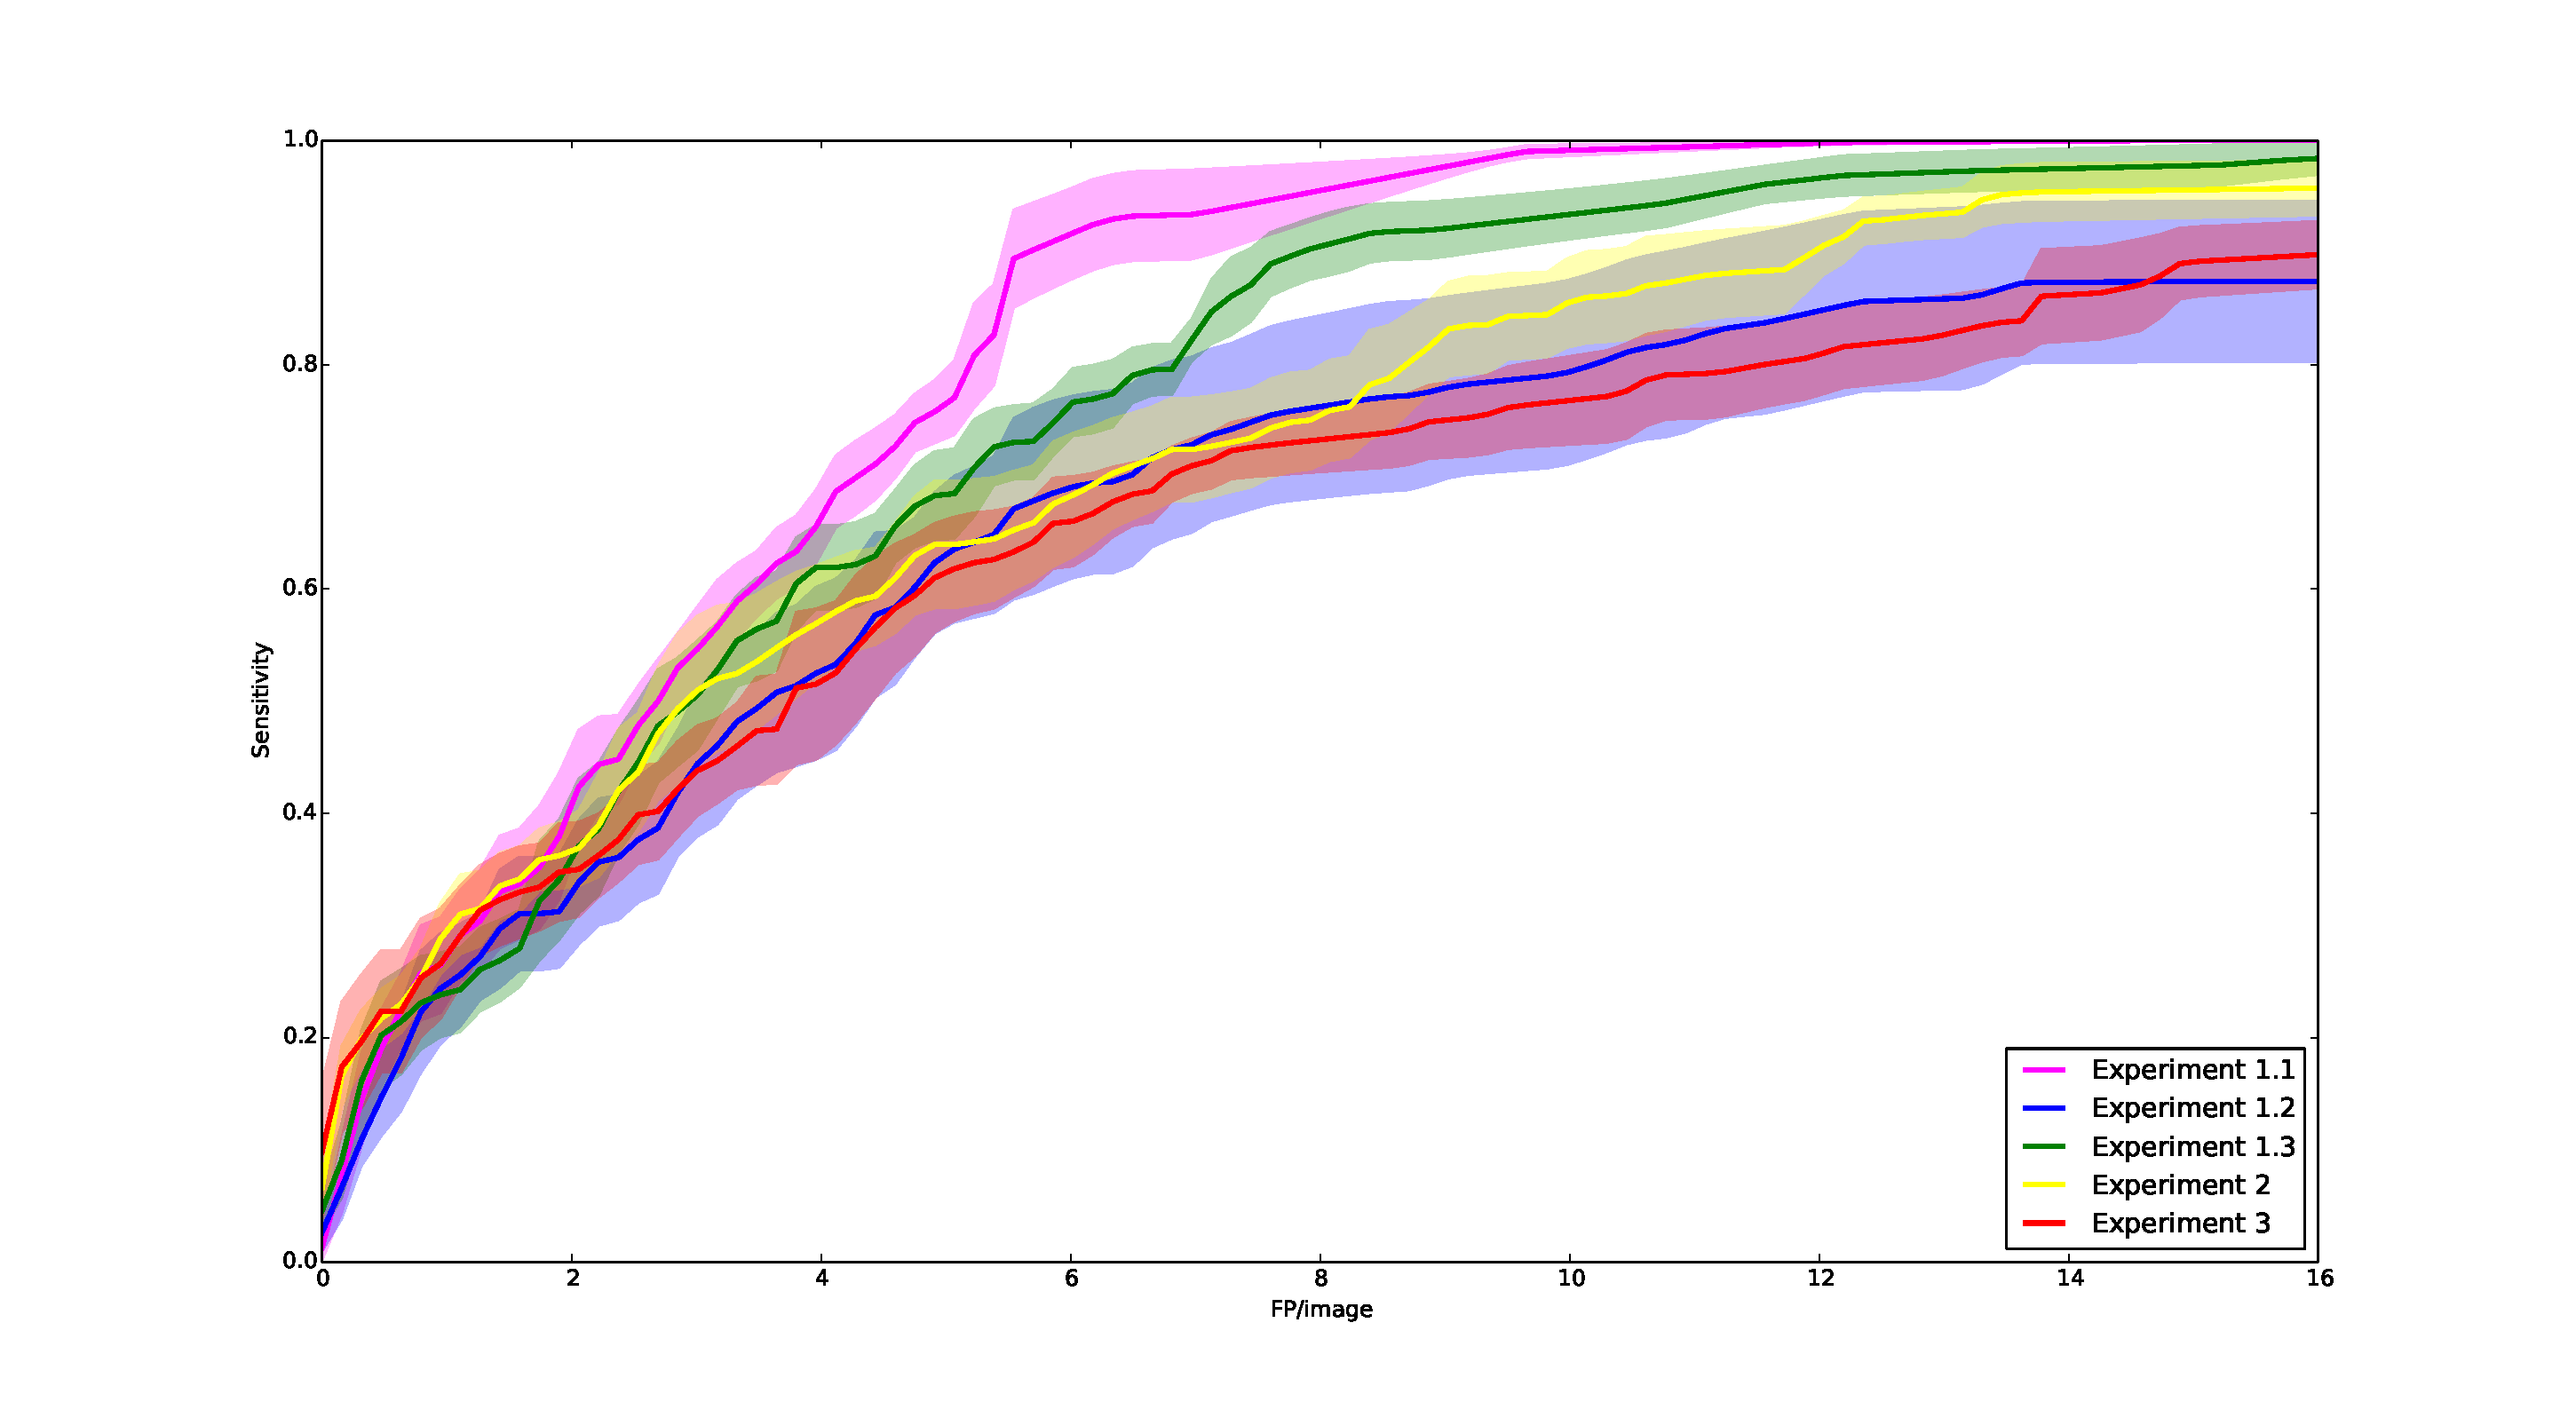
\includegraphics[width=\textwidth]{plots/FROC_plus_std.pdf}
	\caption[FROC curves]{Average FROC curves for every model. Shaded areas represent one standard error of the mean.}
	\label{fig:FROCResults}
\end{figure}

To better analyze our models we look at IOU as the probability threshold varies (Fig.~\ref{fig:IOUResults}): as expected, IOU starts at zero, increases gradually and decreases again as models go from predicting nothing as positive (low intersect) to predicting everything as positive (high union). Overall, curves for models 2 (yellow) and 3 (red) peak higher than those for other models, likely because they learn better feature representations. Model 1.1 (magenta), which is the only one that does not use a weighted function, performs better at lower thresholds because it only predicts low probabilities (less than 0.3); it is also the poorest performer, contrary to what the FROC curve may imply.
\begin{figure}[h]
	\centering
		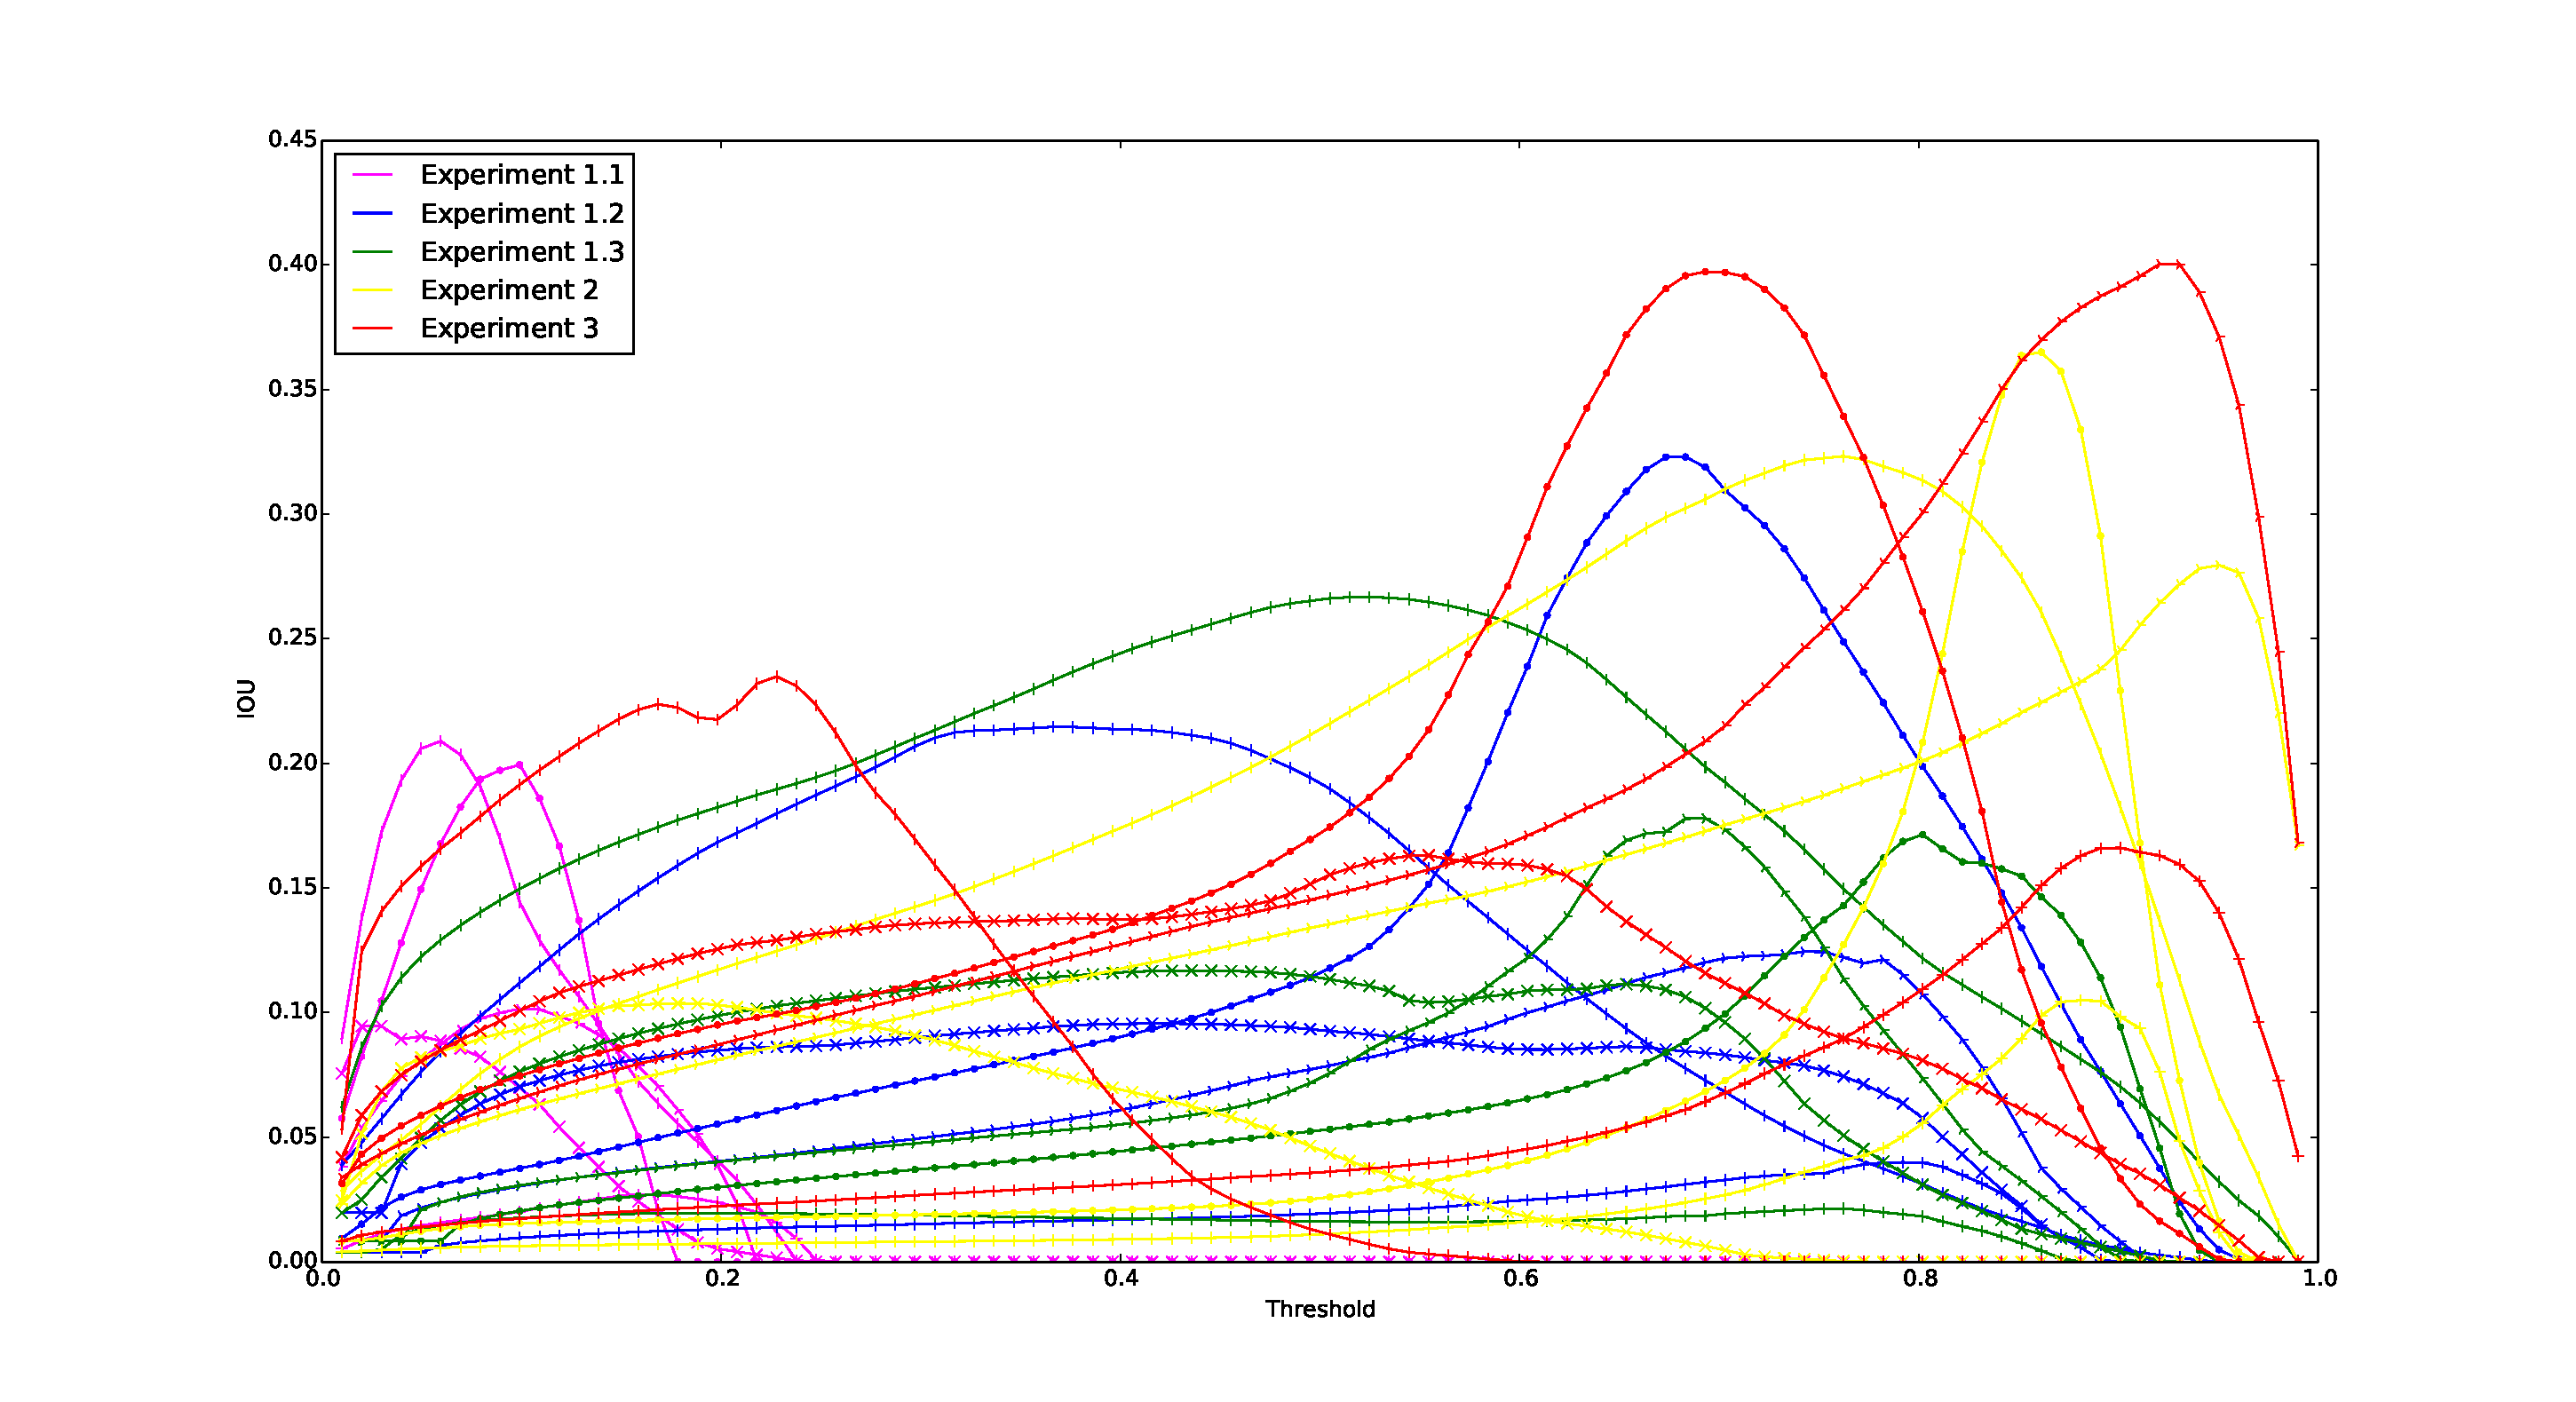
\includegraphics[width=\textwidth]{plots/IOU_all_folds.pdf}
	\caption[IOU curves]{IOU curves for every model and fold for varying probability thresholds. Experiments are drawn in different colors and markers are used to differentiate among folds.}
	\label{fig:IOUResults}
\end{figure}


%The highest peak in each curve represents the best possible IOU that a model could achieve.
%Peaks in each curve represent the best possible IOU that the model could achieve.
The highest peak in each curve represents the best possible IOU that a model achieves in that fold. Although this number is not valid on its own as, beforehand, we ignore what threshold produces it, it is a good proxy for performance and could be used to compare between models. We list these values in Table~\ref{tab:PeakIOUResults}. Once more, models 2 and 3 outperform the simpler architecture with model 3 producing the best results. Comparing experiments 1.1, 1.2 and 1.3, we notice that adding a weighted loss function improves performance while enhancing the images has little effect and may even be detrimental.
%The difference in average performance across folds (last row) shows that, even for the same model, some folds have better (or worse) results. 
The difference in average performance across folds (last row) shows that results also depend on the specific fold used. 
This variability would decrease if we used bigger test sets.
%This difference shrinks for bigger test sets.
\begin{table}[h]
	\centering
	\begin{tabular}{l*{6}{c}}
		\hline
		 & \textbf{Fold 1} & \textbf{Fold 2} & \textbf{Fold 3} &\textbf{Fold 4} &\textbf{Fold 5} & \textbf{Average $\pm$ SEM} \\
		\hline 
		Experiment 1.1	&0.03	&0.09	&0.21	&0.20	&0.10	&0.13 $\pm$ 0.03\\
		Experiment 1.2	&0.04	&0.10	&0.21	&0.32	&0.12	&0.16 $\pm$ 0.04\\
		Experiment 1.3	&0.02	&0.12	&0.27	&0.17	&0.18	&0.15 $\pm$ 0.04\\
		Experiment 2	&0.11 	&0.10	&\textbf{0.32}	&0.37	&0.28	&0.24 $\pm$ 0.05\\
		Experiment 3	&\textbf{0.17}	&\textbf{0.17}	&0.23	&\textbf{0.40}	&\textbf{0.40}	&0.27 $\pm$ 0.05\\
		Average			&0.07		&0.11	&0.25	&0.29	&0.22 &\\
		\hline
	\end{tabular}
	\caption[Peak IOU values for the final models]{Best possible IOU for each experiment. Best model in each column is shown in bold. SEM stands for standard error of the mean.}
	\label{tab:PeakIOUResults}
\end{table}

Lastly, we examine predictions made by our models to get a sense of their qualitative value (Appendix~\ref{app:examples}).
Models predict visually similar heatmaps but different models appear to produce better predictions for particular examples. Models 1.1, 1.3 and 3 are consistently good. On the downside, all models mark chest muscle with high probability and none is particularly good at localizing subtle lesions. It is also notable that model 1.1 is very conservative in its predictions while model 2 is quite more liberal, predicting large areas as probable masses.

\section{Discussion}
We found that convolutional networks are able to segment breast cancer masses as a single end-to-end model going from the original mammograms to a full-size prediction; this simplifies the complex pipeline of analysis used for current computer vision systems. We expect medical image analysis to benefit from adopting modern machine learning techniques to complement or replace more established systems. This work is a step in that direction and, to the best of the author knowledge, the first documented use of convolutional networks for breast cancer lesion segmentation.

Architectures with many layers and a high number of parameters produced the best results regardless of the exact details; however, overfitting started to show in some of our bigger models. Networks with sufficient power were able to learn the complex features needed for this task with realtive ease. Most networks were resilient to changes in th regularization hyperparameter with slightly more work needed to select a learning rate with good convergence properties. Furthermore, using a weighted loss function made training more stable by allowing the network to focus on correctly classifying masses rather than that; this also generated networks who gave predictions in  the complete zero to one range rather than only on the lower side of the scale. Most models did not benefit from enhancing the input images, producing better results for unpreprocessed images. We beleive complex networks benefit from details in the image that were sometimes lost in the preprocessing step. Lckily, This is encouraging given that the goal of this work was to get rid of as many possible steps. produce lesion segmentations in a single learnable step without need of expertise or particular care. And that goal was achieved.

This results agree with many of the positive results achieved in machine learning and medical imaging where convolutional networks as well as other deep learning models have shown succesful results. And some of the more succesful models have started to be deployed for public use both on commercial and medical settings.

Tha main limitation of this work is the small size of our dataset which resulted in small test sets, which in turn gave performance estiomates with high variance difficulting conclusions and assignnig responability. It could also be said that the performance of the network is below that of other more complex systems used for this task, although it is hard to directly compare given the different ways metrics are computed. Both of this limitations could be solved usiung a bigger data set to provide more estable estimates of performance and give more examples for the network to learn. We attest here a proof-of-principle and it is succesful but more research is definitely neede both to confirm the insights obtained in this work and to implement a functional system that could be deployed in real systems. % the way we test things is also weird.

A question left unanswered is whether convolutional networks will be able to exmploit the ability to see more data or whether we will need to enrich our data with other lesions or with breast density to. Given their succesful application inother data-rich setting we believe that convolutional networks are flexible enough to perform much better than presented here and we definitely encourage further work in this direction.

The significance of this works relies on the promise that machine learning systems could improve the performance of current systems and the impact that a small percentage of benefit could have for millions of women. Having a system performing at human or super-human level, as some convolutional networks do in other computer vision tasks, could really improve the rate of detection, be helpful to radioogist and help people in places where it may be hard to get specialized medical attention. We expect machine learning systems to play a role in this quest.

\section{Summary}
All models produced good results with complex architectures performing slightly better. Using a weighted loss function to give more weight to errors committed on breast masses helped both with training and results but using the simple form of image enhancement we use here did not. Results look promising but more research is needed before we can replace entire mammographic systems with a single convolutional network.
